\documentclass{article}
\usepackage{enumerate}
\usepackage{listings}
\usepackage{color}
\usepackage{hyperref}
\usepackage{graphicx}
\usepackage{amsmath}
\graphicspath{ {images/} }
\definecolor{dkgreen}{rgb}{0,0.6,0}
\definecolor{gray}{rgb}{0.5,0.5,0.5}
\definecolor{mauve}{rgb}{0.58,0,0.82}
\def\lc{\left\lceil}   
\def\rc{\right\rceil}


\lstset{
  language=Ruby,
  aboveskip=3mm,
  belowskip=3mm,
  showstringspaces=false,
  columns=flexible,
  basicstyle={\small\ttfamily},
  numbers=none,
  numberstyle=\tiny\color{gray},
  keywordstyle=\color{black},
  commentstyle=\color{black},
  stringstyle=\color{black},
  breaklines=true,
  breakatwhitespace=true,
  tabsize=3
}


\begin{document}
\title{Exploring Deep Learning concepts using Tensorflow on the MNIST dataset}

\author{Torumoy Ghoshal \\ PhD Student\\ Department of Computer and Information Science \\ University of Mississippi}
\maketitle

\section*{Introduction}
Deep learning models have received considerable attention from researchers in the fields of machine learning, statistics, computer vision and so on in the recent times. Deep learning models represent data with multiple levels of abstraction by using multiple processing layers. Each processing layer learns from the previous layer to compute and find a better representation of the data. Backpropagation algorithm is used to change the internal parameters as the model keeps learning over iterations. In doing so, it is expected that some  intricate structure in the data will be represented by the deep learning model.

Depending on the number of neurons and how they are connected, many types of deep learning models can be designed. The models that have found to be very useful are Convolutional Neural Network (CNN) and Recurrent Neural Network (RNN). "Deep convolutional nets have brought about breakthroughs in processing images, video, speech and audio, whereas recurrent nets have shone light on sequential data such as text and speech$^{[1]}$."

"Deep learning methods are often looked at as a black box, with most confirmations done empirically, rather than theoretically.$^{[3]}$" Many aspects of deep learning models are under-researched. To define the theory behind deep learning models, the first step can be performing experiments and discover new properties of the model. This was our motivation to perform a number of experiments in the course of my independent study. We used Google's deep learning framework, Tensorflow, and experimented on the well known MNIST dataset using some implementations of CNN.

\section*{Convolutional Neural Network (CNN)}
\textit{[most of content in this subsection has been collected from $^{[2]}$]}
\newline
\newline
"Convolutional Neural networks, also known as Convolutional Networks (LeCun, 1989), are a specialized kind of neural network for processing data that has a known, grid-like topology. The name "convolutional neural network" indicates that the network employs a mathematical operation called convolution. Convolutional networks are simply neural networks that use convolution in place of general matrix multiplication in at least one of their layers$^{[2]}$." The definition of convolution in deep learning differs slightly from its definition in engineering or pure mathematics. Several variants of convolution function are used in the network. Usually the convolution layer is followed by a RELU layer and a pooling layer.

Mathematically convolution operation is defined as:
$$s(t) = \int x(a)w(t-a)da$$
And typically the convolution operation is denoted with an asterisk:
$$s(t)=(x\ast w)(t)$$
In convolution network terminology, the first argument to the convolution is often referred to as the \textbf{input} and the second argument as the \textbf{kernel}. The output is sometimes referred to as the \textbf{feature map} $^{[2]}$.

The input is usually a multidimensional array of data and the kernel is usually a multidimensional array (tensors) of parameters that are adapted by the learning algorithm. 

We often use convolutions over more than one axis at a time. If we use a two-dimensional image \textit{I} as our input, we may want to use a two dimensional kernel \textit{K}. 

$$S(i,j) = (I \ast K)(i,j) = \sum_{m}^{} \sum_{n} I (m,n) K (i-m, j-n)$$
Since convolution is commutative, the formula can be rearranged as:
$$S(i,j) = (K \ast I)(i,j) = \sum_{m}^{} \sum_{n} I (i-m, j-n)K (m,n) $$
A variation of the above equation is usually implemented in most machine learning libraries.

"Any neural network algorithm that works with matrix multiplication and does not depend on specific properties of the matrix structure should work with convolution, without requiring any further changes to the neural network $^{[2]}$."
\begin{center}
	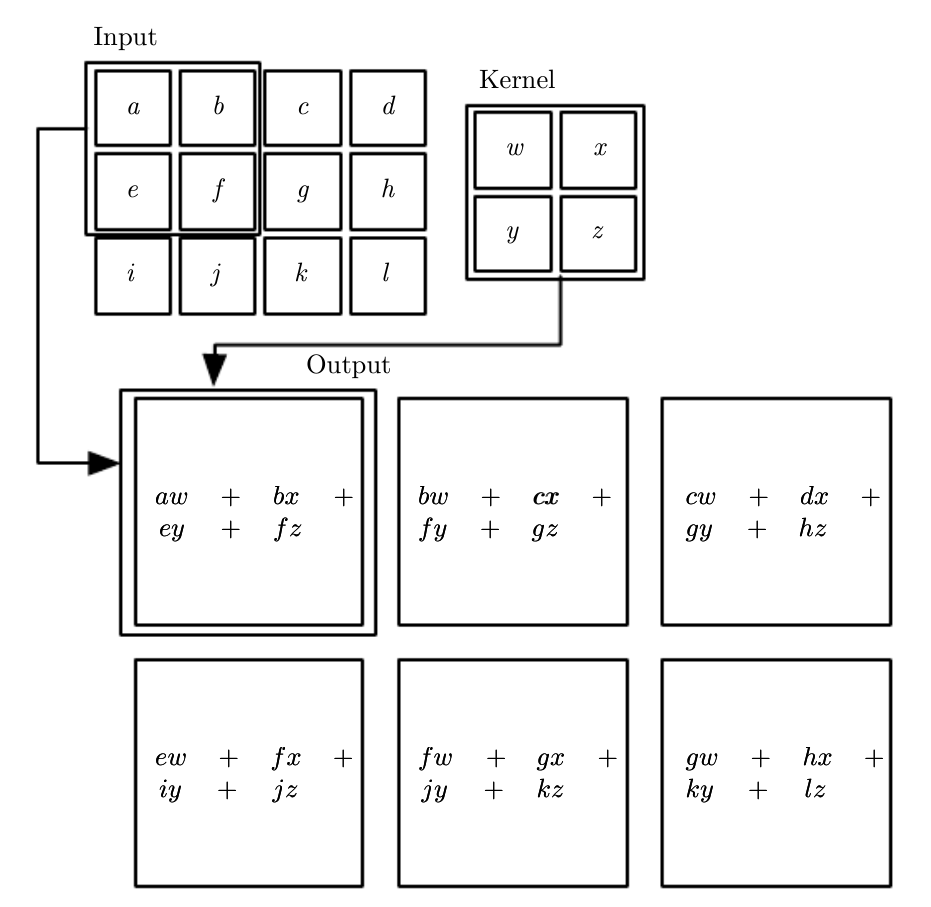
\includegraphics[scale=0.2]{convolution}
\end{center}
The above represents a 2-D convolution operation usually utilized in a neural network without kernel flipping. The output is restricted to only the positions where kernel stays within the image. This is also known as 'valid' convolution. 

The convolution operation is usually followed by RELU which is a non-linear activation function. The function is given by:
$$f(x) = Max(0, x)$$
The following figure shows how the RELU function works:
\begin{center}
	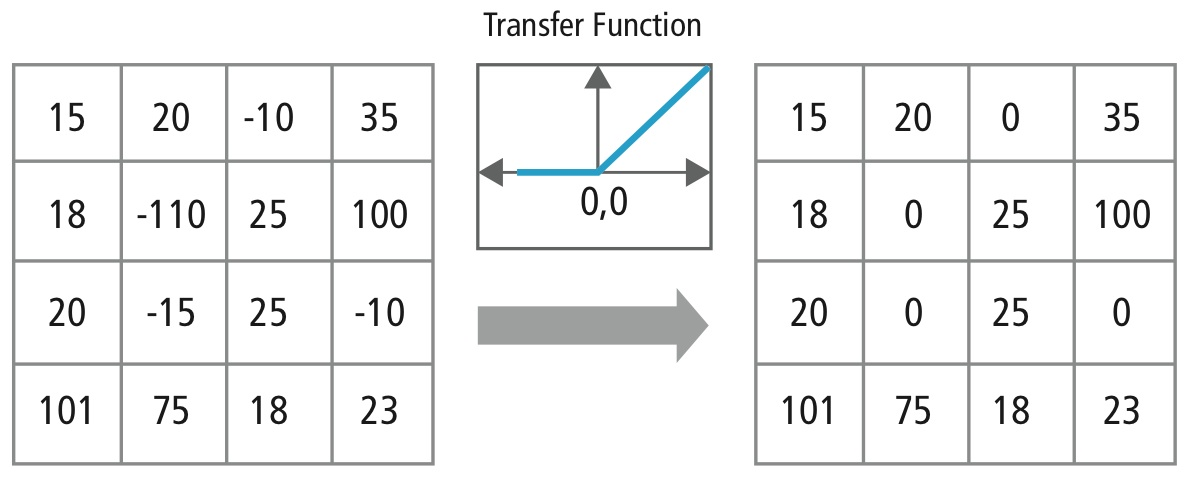
\includegraphics[scale=0.2]{relu}
\end{center}
\begin{center}
		\textit{[Image source: ${[4]}$]}
\end{center}
The RELU function replaces the non-negative values with 0. After the RELU operation a pooling layer is applied. "Pooling layer partitions the input image into a set of non-overlapping rectangles and, for each such sub-region, outputs the maximum. The intuition is that the exact location of a feature is less important than its rough location relative to other features. The pooling layer serves to progressively reduce the spatial size of the representation, to reduce the number of parameters and amount of computation in the network, and hence to also control overfitting${[6]}$."
\begin{center}
	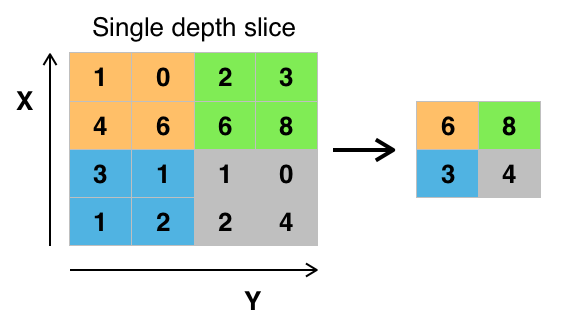
\includegraphics[scale=0.2]{max_pooling}
\end{center}
\begin{center}
	\textit{[Image source: ${[5]}$]}
\end{center}
The overall convolution process can be represented as:
\begin{center}
	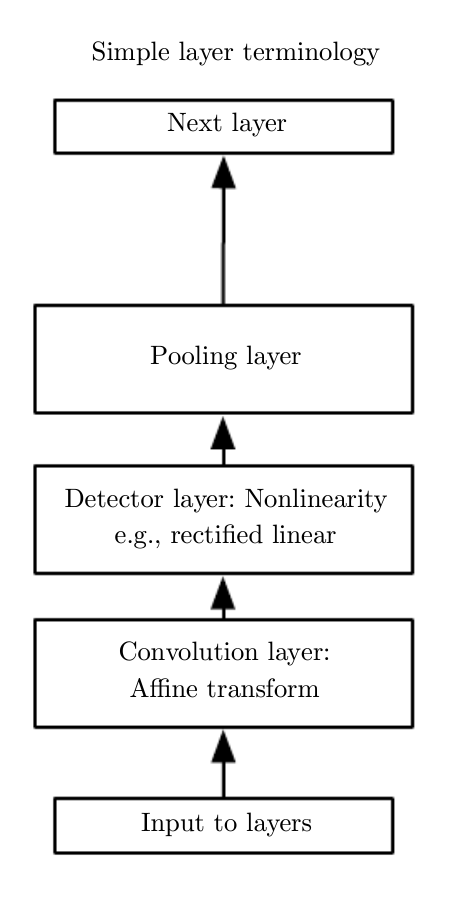
\includegraphics[scale=0.2]{diagram}
\end{center}
\begin{center}
	\textit{[Image source: ${[2]}$]}
\end{center}

In practice, a number of such layers are applied. Using 3 such layers is very common. The last convolution layer is followed by a fully connected layer and then \textit{Softmax} algorithm is applied to decided a winner. The overall convolution neural network can be represented as below:

\begin{center}
	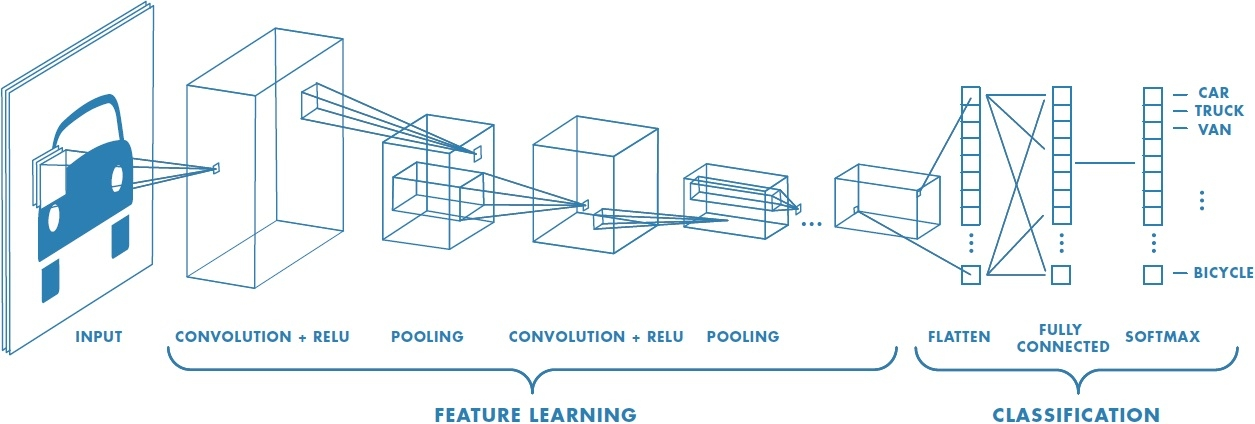
\includegraphics[scale=0.28]{cnn}
\end{center}
\begin{center}
	\textit{[Image source: ${[7]}$]}
\end{center}

Dropout is often applied in the convolution layers and the fully connected layer. Dropout is a technique to address over-fitting in very large neural networks. "During training, dropout samples from an exponential number of different “thinned” networks. At test time, it is easy to approximate the effect of averaging the predictions of all these thinned networks by simply using a single unthinned network that has smaller weights. This significantly reduces overfitting and gives major improvements over other regularization methods"$^{[10]}$.

\begin{center}
	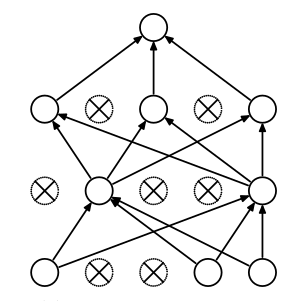
\includegraphics[scale=0.5]{dropout}
\end{center}

\section*{Experiment Setup}
Source code was first obtained from ${[8]}$. The code was then significantly modified so that any dataset can be used without having to change the code much every time. Initially a laptop with Intel Core i5 processor and 8 GB ram was used. The CNN implementation takes roughly 35 mins for 20000 iterations on the MNIST dataset on the laptop. This proved to be inconvenient for experiments. Later clusters on the Mississippi Center for Supercomputing Research (MSCR)$^{[9]}$ were used which sped up the operation significantly. It took 3 to 5 mins for 20000 iterations fro CNN on the MNIST dataset.

Many smaller datasets of smaller size were obtained from the dataset. The size varied from 5000 samples to 50000 samples with random shuffling. All of experiments were tested on a separate test dataset that contained 10000 samples.

\section*{Experiments and Results}
\subsection*{CNN on pure MNIST dataset}
\textbf{Motivation:} The motivation behind our first experiment was to test the hypotheses that Deep Neural Networks benefit from a larger sample size. 
\begin{center}
	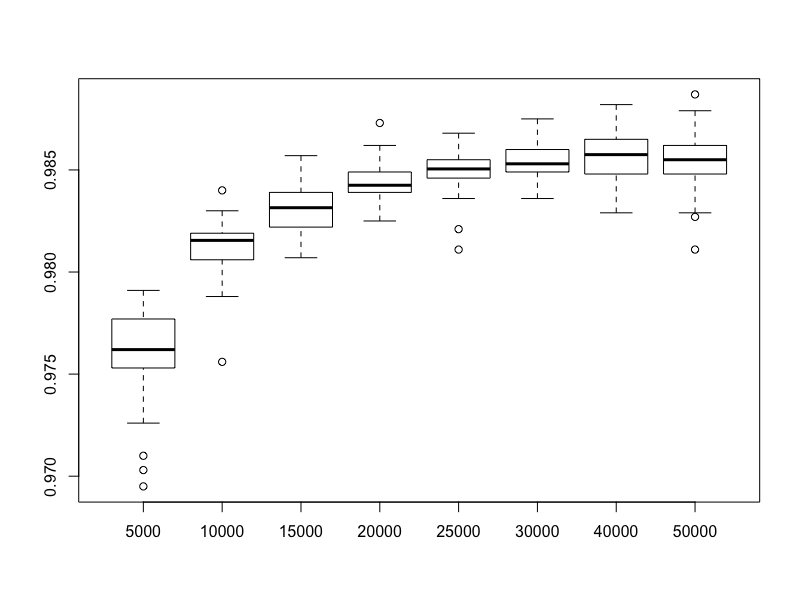
\includegraphics[scale=0.35]{new_cnn_mnist_pure}
\end{center}
\begin{center}
	Fig: Boxplot of Accuracy graph of CNN on the pure MNIST dataset. The \textit{X} axis represents sample size and \textit{Y} axis represents accuracy.
\end{center}

The word \textit{Pure} indicates that the samples were not altered in any way. This is mentioned because we also conducted experiments where we applied permutation matrix to the dataset. In those cases the dataset will be referred to as \textit{Permuted}.

\textbf{Analysis:} In the figure above, it can be observed that we have achieved accuracy close to $98.6\%$. Accuracy increased with the increase in sample size. Though the range is small ($1\%$), the increase in accuracy could be noticed. The graphs represent the average after 30 runs of CNN on the corresponding size.

\subsection*{CNN on EMNIST dataset}
\textbf{Motivation:} Whereas MNIST dataset consists of images of handwritten digits, EMNIST dataset consists of handwritten characters. Our goal was to see a similar curve as seen on the MNIST dataset. This would prove the CNN benefits from more samples.

\begin{center}
	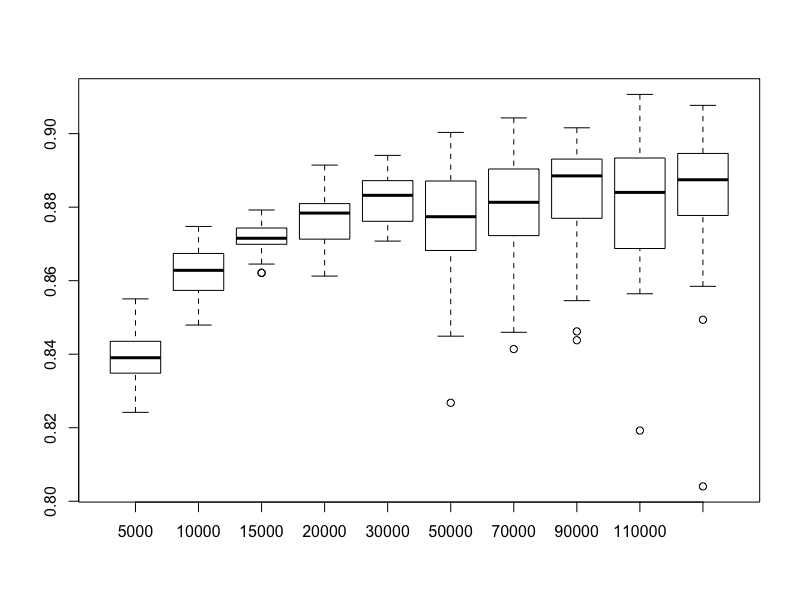
\includegraphics[scale=0.35]{EMNIST_pure_CNN}
\end{center}
\begin{center}
	Fig: Boxplot of Accuracy graph of CNN on the EMNIST dataset.
\end{center}

\textbf{Analysis:} The graph looks similar to MNIST dataset, but accuracy was less. This was because we had to work with more classes compared to the MNIST dataset. However, this time range was higher, roughly from $83\%$ to $89\%$.

\subsection*{Random Forest and SVM on pure MNIST}
\textbf{Motivation:} We wanted to see how other popular machine learning algorithms performed compared to CNN. We chose Random Forest and Support Vector Machine (SVM) for this experiment.
\begin{center}
	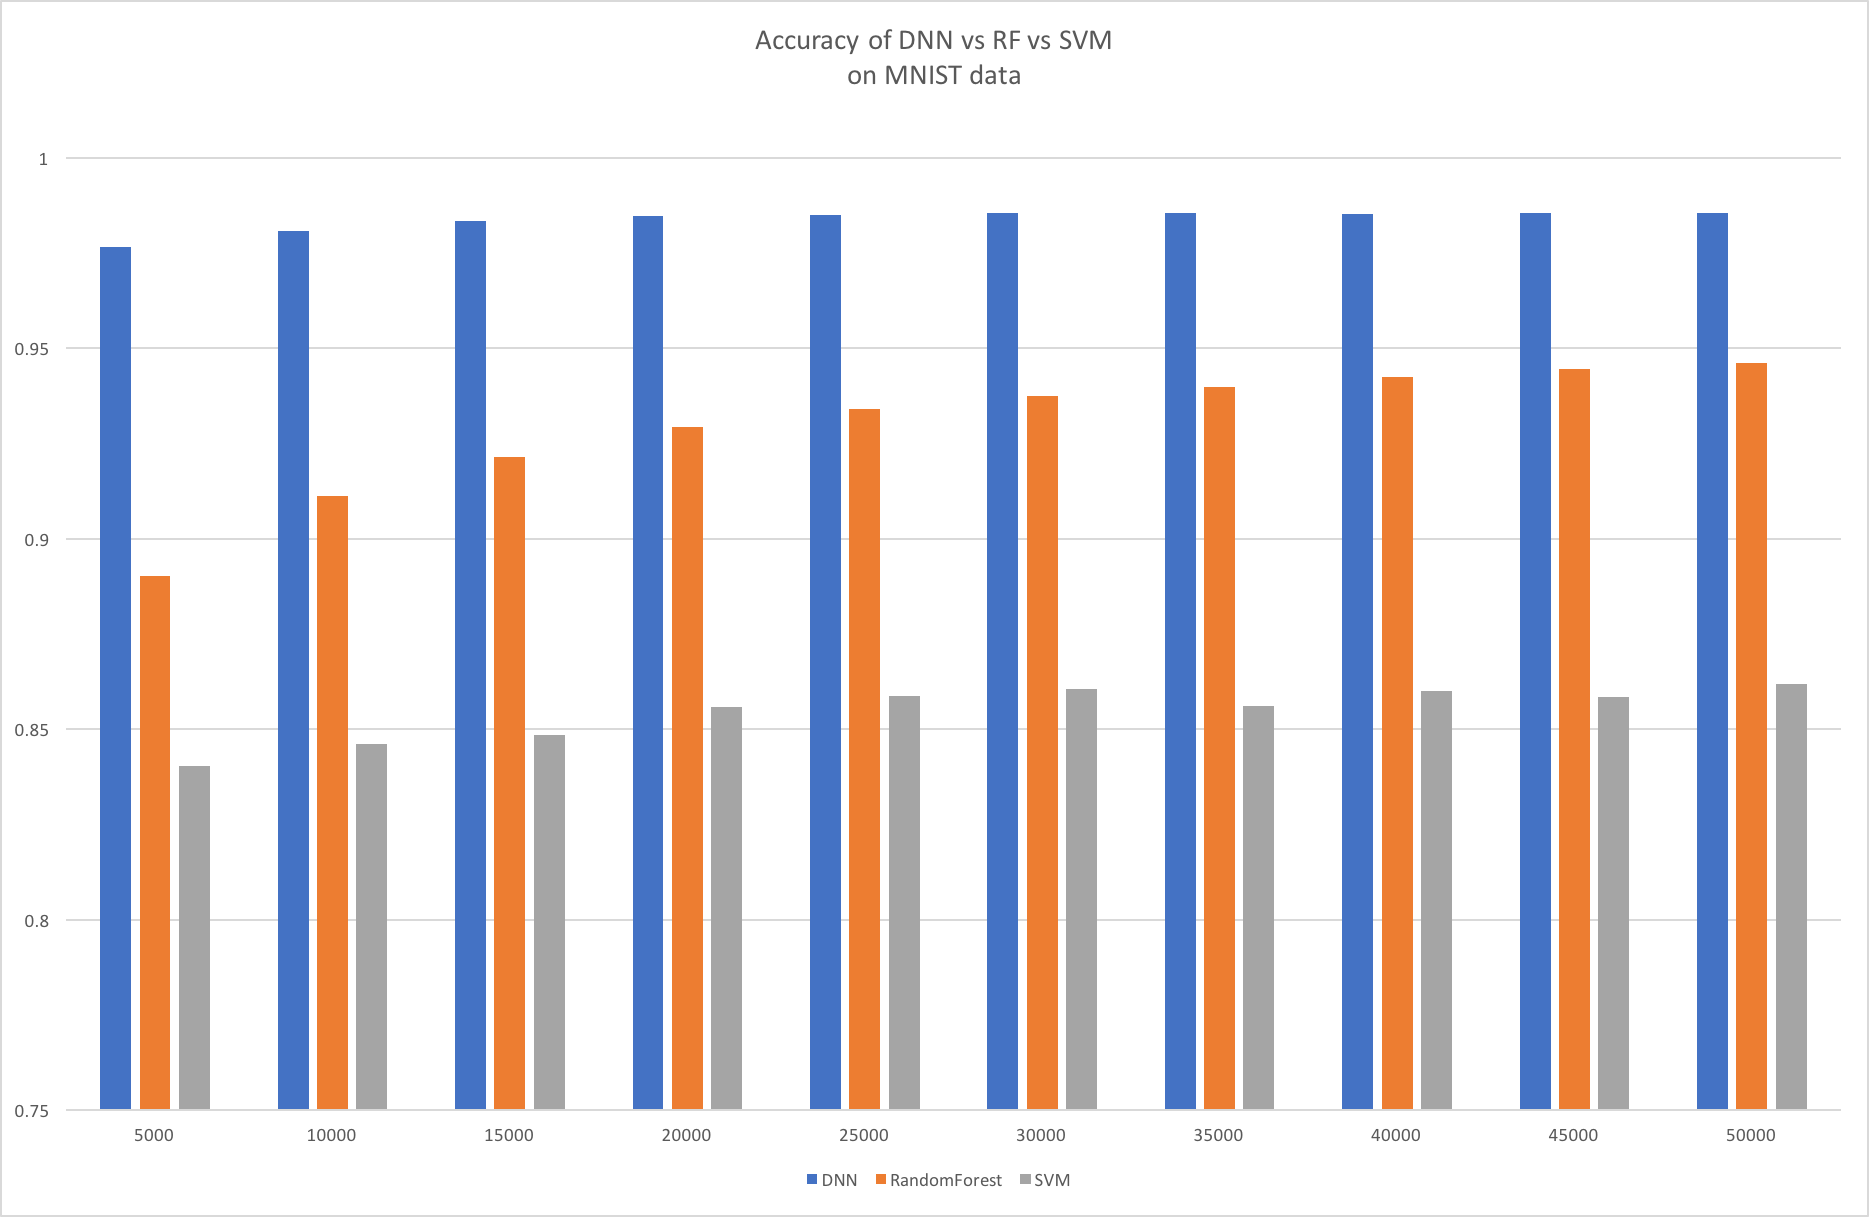
\includegraphics[scale=0.35]{DNN_RF_SVM}
\end{center}
\begin{center}
	Fig: Accuracy graph of CNN, Random Forest and SVM on the pure MNIST dataset
\end{center}

\textbf{Analysis:} As expected, CNN performed the best. However, performance of Random Forest was very good. This suggests that if time requirement is more important than accuracy, then RF can be used. This will not guarantee the best result, but it will guarantee good enough result in a much shorter time.


\subsection*{Multi-layer network on pure MNIST}
\textbf{Motivation:} We wanted to see if the high accuracy of CNN was because it was a Deep Neural Network or because it had the convolution property. To do that, we removed the convolution property from the network and implemented a 5 layer network in which the last layer is a \textit{Softmax} layer.
\begin{center}
	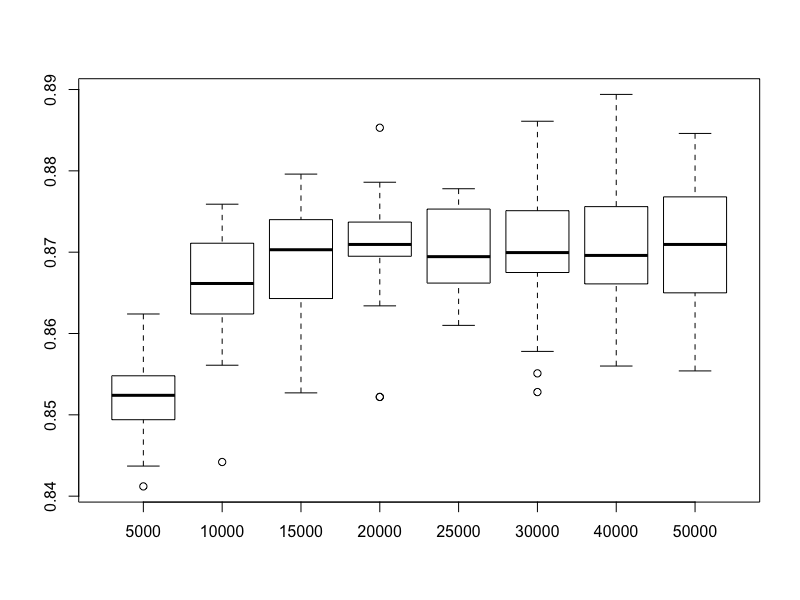
\includegraphics[scale=0.35]{Perceptron_MNIST_CNN}
\end{center}
\begin{center}
	Fig: Accuracy graph of a 5-layer network on the pure MNIST dataset
\end{center}

\textbf{Analysis:} Accuracy was much less compared to CNN. This led to our conclusion that the high accuracy was achieved because CNN could take advantage of the spatial property of the dataset. It should also be noted that the performance was worse than RF on the same dataset.

However, this graph is not conclusive. Tuning the architecture and learning parameters could give better accuracy. But there is no clear way to do that.

\subsection*{CNN on permuted MNIST}
\textbf{Motivation:} The motivation for this experiment came from the previous experiment. As we concluded that CNN benefits from the spatial property, we expected that if we can destroy the spatial property, the performance should drop. To do that we applied two permutation matrices \textit{P1}, \textit{P2} to all the training samples and test samples. There were two cases:
\begin{enumerate} [a.]
	\item P2 = inverse(P1)
	\item P2 != P1
\end{enumerate}
\begin{center}
	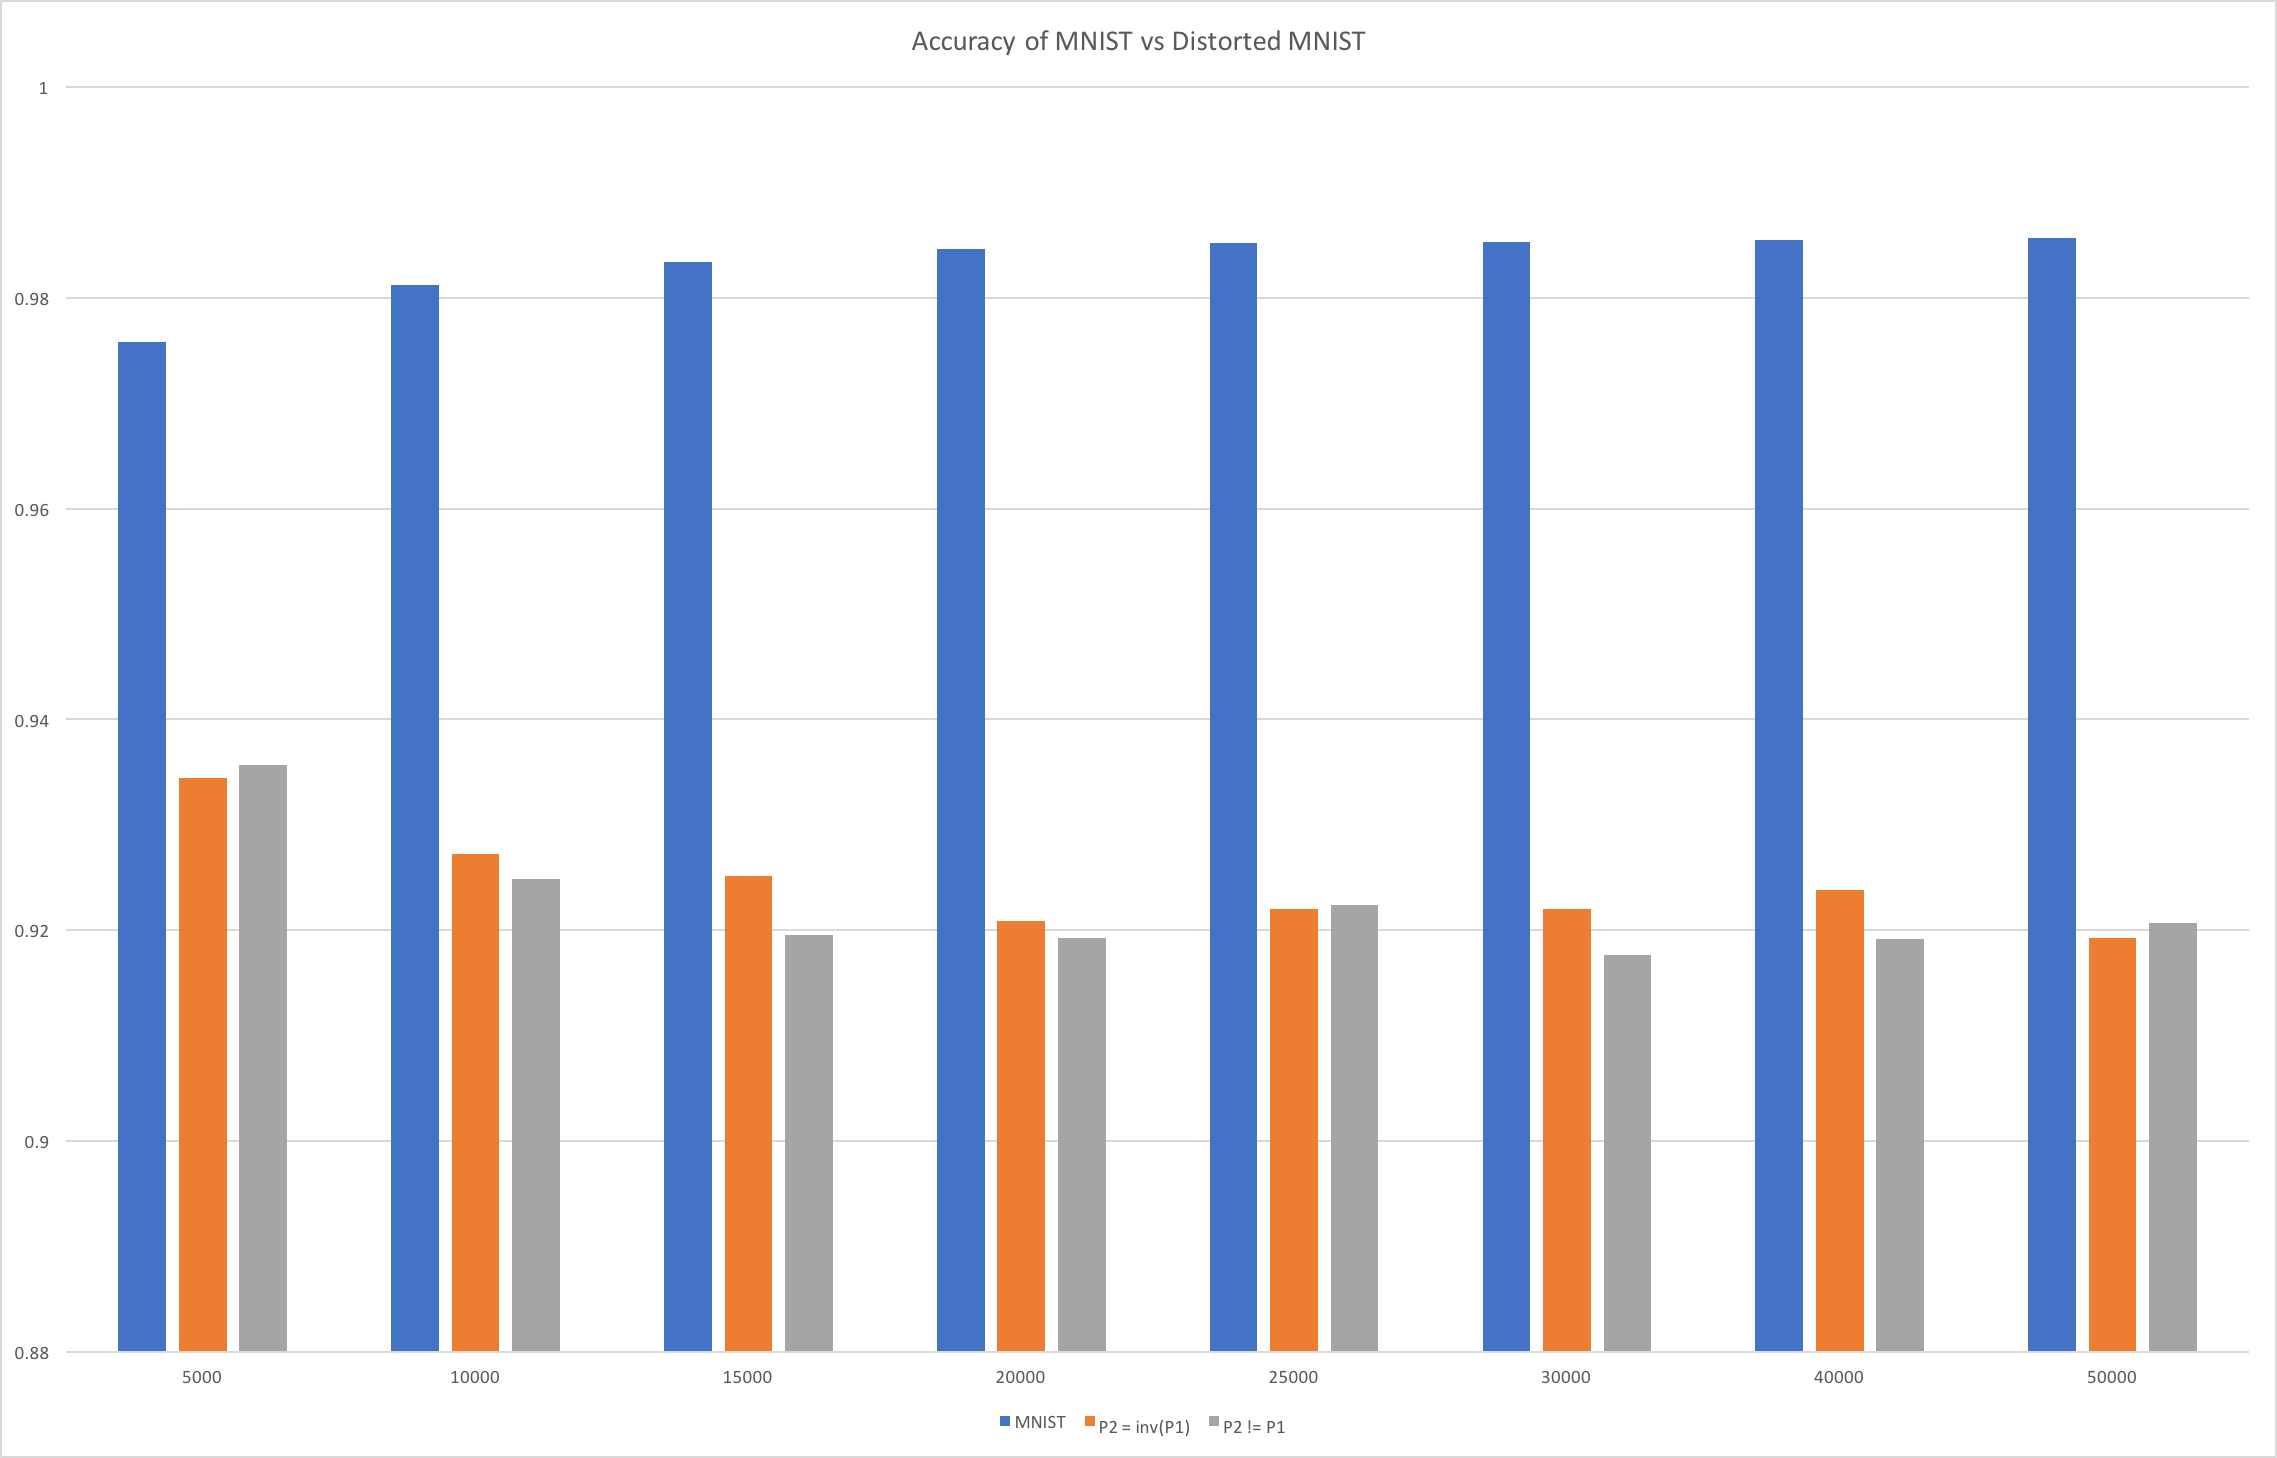
\includegraphics[scale=0.3]{Accuracy_graph}
\end{center}
\begin{center}
	Fig: Accuracy graph of CNN on permutated MNIST vs pure MNIST
\end{center}
We can look at the experiment more closely on the following boxplot:
\begin{center}
	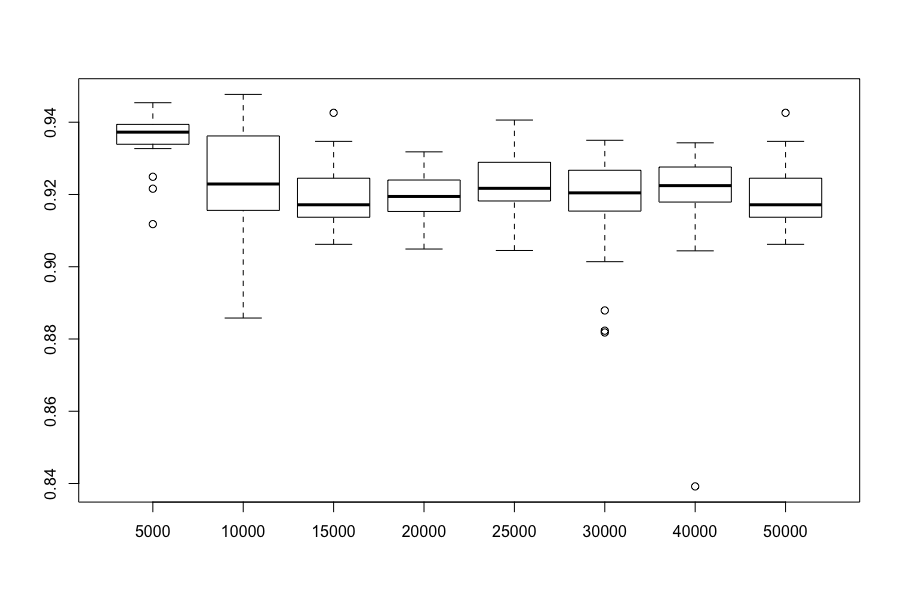
\includegraphics[scale=0.35]{mnist_permutated_cnn}
\end{center}
\begin{center}
	Fig: Boxplot of CNN on permuted MNIST
\end{center}

\textbf{Analysis:} As expected, performance dropped. However, the accuracy of around $92\%$ is still quite high.

\subsection*{RF on permuted MNIST}
\textbf{Motivation:} We wanted to see how RF perform on the permuted dataset. The expectation was that RF performance should not depend on the spatial property. Hence, accuracy graph should look similar to the one for pure MNIST.
\begin{center}
	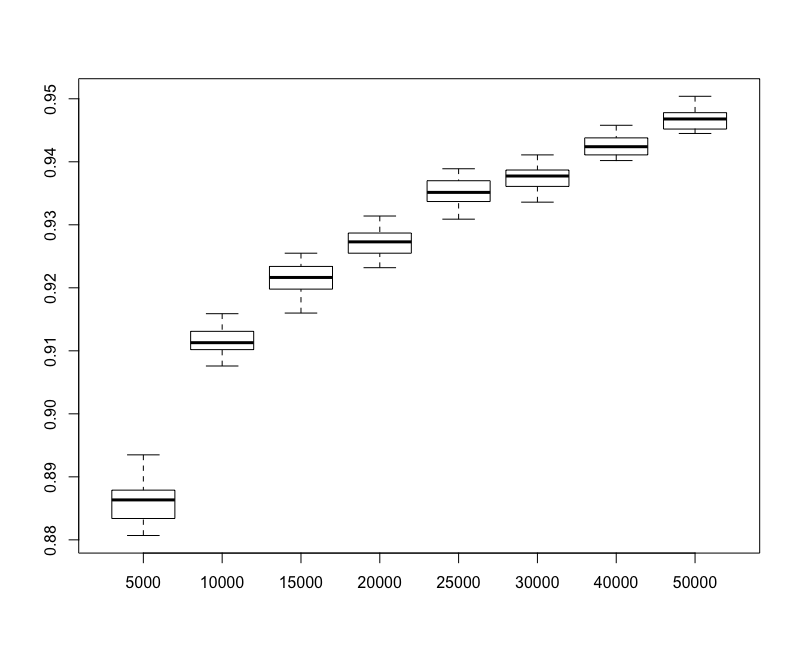
\includegraphics[scale=0.35]{rf_permuted}
\end{center}
\begin{center}
	Fig: Boxplot of RF on permuted MNIST
\end{center}

\textbf{Analysis:} As expected, performance has remained similar. So we can conclude RF perform equally well for cases when spatial property exists and when it does not.


\section*{Conclusion and Future Work:}
In a number of projects, we verified some properties of CNN. Though the success of CNN is remarkable in some cases, unless we truly understand all of its properties, we cannot guarantee such success. Deep Learning as a whole still remains a 'blackbox' model. Unless we do more experiments and define all the theories and rules, working with deep learning models will remain a 'trial and error' process. We hope to do more work to define theories and rules that make deep learning models more usable.

\section*{Acknowledgment}
I would like to thank Dr. Yixin Chen of Dept. of Computer and Information science, University of Mississippi, for giving me countless ideas for most of the projects and advising me throughout the semester. I would also like to thank Dr. Dawn Wilkins for giving me valuable suggestions and Dr. Yunyun Zhou for the same and helping me setup an account with MCSR. I am also thankful to all the members of the machine learning research group.

\section*{References:}
\begin{enumerate}
\item Yann LeCun, Yoshua Bengio \& Geoffrey Hinton, "Deep learning", page: 436, NATURE, Vol 521, 28 May 2015
\item Ian Goodfellow,‎ Yoshua Bengio,‎ Aaron Courville, "Deep Learning (Adaptive Computation and Machine Learning series)", The MIT Press, ISBN 978-0262035613
\item Knight, Will (2017-03-14). "DARPA is funding projects that will try to open up AI's black boxes". MIT Technology Review. Retrieved 2017-11-02.
\item https://www.embedded-vision.com/platinum-members/cadence/embedded-vision-training/documents/pages/neuralnetworksimagerecognition
\item https://upload.wikimedia.org/wikipedia/commons/e/e9/Max\_pooling.png
\item https://en.wikipedia.org/wiki/Convolutional\_neural\_network\#Pooling\_layer
\item https://www.mathworks.com/content/mathworks/www/en/discovery/convolutional-neural-network/jcr:content/mainParsys/image\_copy.adapt.full.high.jpg/1508999490138.jpg
\item https://github.com/tensorflow/tensorflow/blob/r1.4/tensorflow/examples/tutorials/mnist/mnist\_deep.py
\item https://mcsr.olemiss.edu/
\item Nitish Srivastava, Geoffrey Hinton, Alex Krizhevsky, Ilya Sutskever, Ruslan Salakhutdinov, "Dropout: A Simple Way to Prevent Neural Networks from Overfitting", Journal of Machine Learning Research 15 (2014) 1929-1958
\item https://lvdmaaten.github.io/tsne/
\end{enumerate}

\end{document}
